\section{Auswertung}
	\label{sec:auswertung}
	Vor allen Messungen musste der Nulleffekt ermittelt werden, um unsere Messwerte sp"ater von diesem zu bereinigen.
	Hierf"ur wurden die Zerf"alle $N_{\mathrm{u}}$, die ohne Probe ermittelt werden, "uber lange Zeit gez"ahlt.
	Anschlie"send konnten die eigentlichen Messungen durch\-ge\-f"uhrt werden.
	

	Um auf die Halbwertszeiten zu schlie"sen konnte die Beziehung \eqref{eqn:t_halb} aus Kapitel \ref{sec:theorie} ver\-wen\-det werden.
	Weil die Messwerte Poisson-verteilt sind, betrug der Fehler auf die Messwerte

	\begin{eqnarray*}
		\Delta N_{\Delta t, \mathrm{gem}} & = & \sqrt{N_{\Delta t, \mathrm{gem}}}, \\
		\Delta N_{\Delta t, \mathrm{u}} & = & \sqrt{N_{\Delta t, \mathrm{u}}},\\
		\Rightarrow \Delta N_{\Delta t} & = & \sqrt{N_{\Delta t, \mathrm{gem}} + N_{\Delta t, \mathrm{u}}} .
	\end{eqnarray*}

	$N_{\Delta t, \mathrm{u}}$ bezeichnet dabei den Nulleffekt pro Messung.
	Um eine Ausgleichsrechnung durch\-zu\-f"uh\-ren wurden die Werte linearisiert, was einen weiteren Fehler durch Gau"s'sche Fehlerfortpflanzung erzeugt:

	\begin{equation*}
		\Delta N_{l} = \frac{\partial}{\partial N_{\Delta t, \mathrm{gem}}} \ln{\left( N_{\Delta t, \mathrm{gem}} - N_{\Delta t, \mathrm{u}} \right)} \cdot \Delta N_{\Delta t} = \frac{\Delta N_{\Delta t}}{N_{\Delta t, \mathrm{gem}} - N_{\Delta t, \mathrm{u}}} .
	\end{equation*}

	Schlie"slich konnte eine lineare Regression mit scipy durchgef"uhrt werden, welche $\lambda$ und somit die Halbwertszeiten $T$ lieferte.

	\subsection{Halbwertszeit von Indium}
		\label{subsec:indium}
		Es wurden 15 Messungen "uber jeweils $\Delta t = \SI{240}{\second}$ durchgef"uhrt.
		Anschlie"send konnte, wie oben beschrieben, durch lineare Regression $T_\mathrm{In}$ ermittelt werden. Es musste dabei wiederum ein Gau"s'scher Fehler ber"ucksichtigt werden:

		\begin{displaymath}
			\Delta T = \left|\frac{\partial T}{\partial \lambda} \cdot \Delta \lambda \right| = \frac{\Delta \lambda}{\lambda^2} \ln{2} ,
		\end{displaymath}

		wobei $\Delta \lambda$ den Fehler der linearen Regression bezeichnet.
		Es ergaben sich die Werte

		\begin{eqnarray*}
			\lambda & = & \SI{18.212 (94)e-3}{\per \second} , \\
			T_\mathrm{In} & = & \SI{3823 (195)}{\second} = \SI{1}{\hour}\,\SI{3.417 (3250)}{\minute} .
		\end{eqnarray*}

		\begin{table}[!h]
			\begin{center}
				\label{tabelle:indium}
				\caption{Messwerte f"ur Indium-116}
				\begin{tabular}{|c|c||c|c|}
					\hline 
					Messung & $N_{\Delta t, \mathrm{gem}}[1 / 240\,\mathrm{s}]$ & Messung & $N_{\Delta t, \mathrm{gem}}[1 / 240\,\mathrm{s}]$\\
					\hline 
					1 & 2265 & 2197 & 9 & 1696 & 1628\\
2 & 2236 & 2168 & 10 & 1613 & 1545 \\
3 & 2243 & 2175 & 11 & 1519 & 1451 \\
4 & 2038 & 1970 & 12 & 1421 & 1353 \\
5 & 1926 & 1858 & 13 & 1412 & 1344 \\
6 & 1875 & 1807 & 14 & 1352 & 1284 \\
7 & 1639 & 1571 & 15 & 1203 & 1135 \\
8 & 1756 & 1688 & & & \\
					\hline 
				\end{tabular}
			\end{center}
		\end{table}

		\begin{figure}[!h]
			\centering
			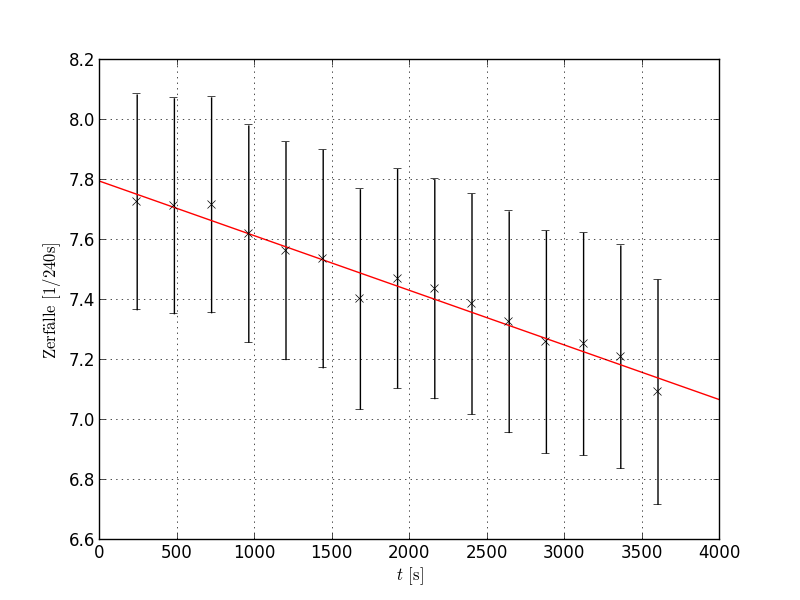
\includegraphics[width = 15cm]{img/graph_indium_linearisiert.png}
			\caption{Bereinigte Messwerte und Graph f"ur Indium-116}
			\label{fig:indium}
		\end{figure}

	\clearpage

	\subsection{Halbwertszeit von Rhodium}
		\label{subsec:rhodium}
		Bei dieser Messung war zu beachten, dass die Probe zwei verschiedene Isotope ${}_{45}^{104}\mathrm{Rh}$ und das angeregte ${}_{45}^{104i}\mathrm{Rh}$ enthielt.
		Weil beide Isotope aber unterschiedliche Halbwertszeiten $T_\mathrm{Rh}$ haben,
		konnte zun"achst, wie in Kapitel \ref{sec:theorie} beschrieben, die gr"o"sere Halbwertszeit $T_{\mathrm{Rh}, 2}$ bestimmt werden.

		Anschlie"send wurden die hierdurch verursachten Zerf"alle von den ersten 19 Messwerten abgezogen und wie in Kapitel \ref{subsec:indium} fortgefahren.

		$T_{\mathrm{Rh}, 1}$ bezeichnet im Folgenden die Halbwertszeit f"ur die ersten 19 Messwerte, also ${}_{45}^{104i}\mathrm{Rh}$ und $T_{\mathrm{Rh}, 2}$ f"ur die letzten 19 Messwerte, also ${}_{45}^{104}\mathrm{Rh}$.

		Zwei mittlere Messwerte wurden ausgelassen, weil die statistischen Schwankungen zu fehlern in der Rechnung f"uhrten.
		\newline


		F"ur ${}_{45}^{104}\mathrm{Rh}$ ergab sich dann

		\begin{eqnarray*}
			\lambda & = & \SI{16.85 (93)e-3}{\per \second} , \\
			T_\mathrm{In} & = & \SI{41.146 (2270)}{\second} .
		\end{eqnarray*}

		F"ur ${}_{45}^{104i}\mathrm{Rh}$ lieferten die Messwerte

		\begin{eqnarray*}
			\lambda & = & \SI{2.418 (840)e-3}{\per \second} , \\
			T_\mathrm{In} & = & \SI{286.63 (9958)}{\second} = \SI{4.78 (66)}{\minute} .
		\end{eqnarray*}

		\clearpage

		\begin{table}[!h]
			\begin{center}
				\caption{Messwerte f"ur Rhodium}
				\label{tabelle:rhodium}
				\begin{tabular}{|c|c||c|c||c|c|}
					\hline 
					Messung & $N_{\Delta t, \mathrm{gem}}[1 / 12\,\mathrm{s}]$ & Messung & $N_{\Delta t, \mathrm{gem}}[1 / 12\,\mathrm{s}]$ & Messung & $N_{\Delta t, \mathrm{gem}}[1 / 12\,\mathrm{s}]$\\
					\hline 
					1 & 449 & 15 & 69 & 29 & 23 \\
2 & 405 & 16 & 72 & 30 & 37 \\
3 & 402 & 17 & 48 & 31 & 25 \\
4 & 356 & 18 & 55 & 32 & 24 \\
5 & 278 & 19 & 51 & 33 & 17 \\
6 & 247 & 20 & 50 & 34 & 19 \\
7 & 165 & 21 & 40 & 35 & 19 \\
8 & 155 & 22 & 30 & 36 & 23 \\
9 & 162 & 23 & 41 & 37 & 30 \\
10 & 142 & 24 & 31 & 38 & 23 \\
11 & 112 & 25 & 46 & 39 & 21 \\
12 & 116 & 26 & 23 & 40 & 25 \\
13 & 97 & 27 & 27 && \\
14 & 83 & 28 & 43 && \\
					\hline 
				\end{tabular}
			\end{center}
		\end{table}

		\enlargethispage{5cm}

		\begin{figure}[!h]
			\centering
			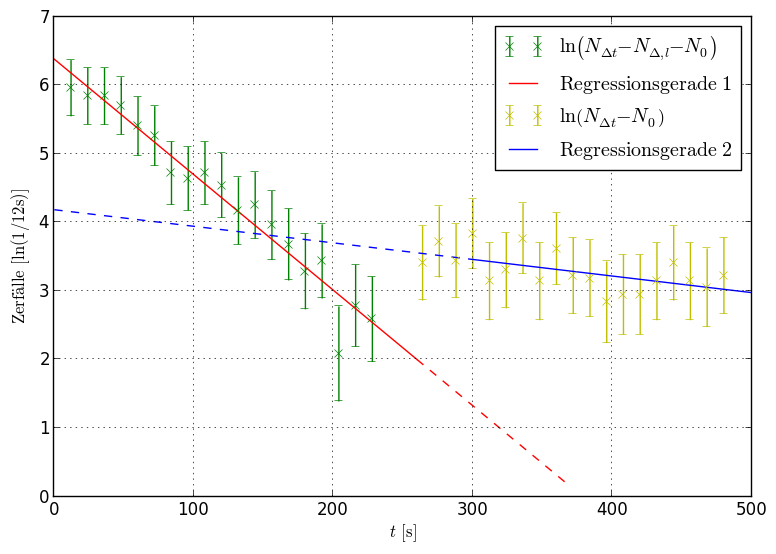
\includegraphics[width = 14cm]{img/graph_rhodium_linearisiert.png}
			\caption{Bereinigte Messwerte und Graph f"ur Rhodium-104 und Rhodium 104i}
			\label{fig:the_label}
		\end{figure}

		\clearpage
